\prob
{\label{t2:p7}
    Let $T_8$ and $R_8$ be the vector matroids of the following matrices over $GF(3)$:\pn
            \begin{center}
                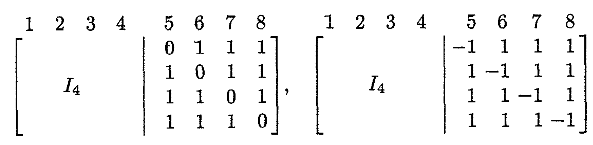
\includegraphics[width=12cm]{Test2/Problem7/FirstMatrices.png}
            \end{center}\pn
    
    \begin{enumerate}[label=(\roman*)]
        \item Show that $T_8$ and $R_8$ ar both self-dual.
        \item Show that $R_8$ is identically self-dual but $T_8$ is not.
        \item Give geometric representation for $T_8$ and $R_8$.
        \item Show that if $M \in \{T_8, R_8\}$ and $X = E(M) \setminus \{8\}$, then
                $(M|X)^* \cong F_7^-$.
        \item Consider the following matrices over $GF(3)$:
            \begin{center}
                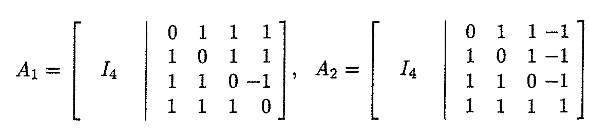
\includegraphics[width=12cm]{Test2/Problem7/SecondMatrices.png}
            \end{center}\pn
            Show, by applying a sequence of the row and clolumn opeartions to $A_1$ and $A_2$
            that $M[A_1] \cong T_8$ and $M[A_2] \cong R_8$.
        \item Show that $R_8$ can be obtained from $AG(3, 2)$ by relaxing two disjoint 
            circuit-hyperplanes.
    \end{enumerate}
}
\begin{proof}$\,$\pn
    \begin{enumerate}[label=(\roman*)]
        \item 
        \item
        \item
        \item
        \item
        \item
    \end{enumerate}
\end{proof}